% ========== HARE ==========
\begin{frame}{%
  \begin{minipage}[c]{0.30\textwidth}
    Hare
  \end{minipage}%
  \hfill
  \begin{minipage}[c]{0.45\textwidth}
    \footnotesize
    \textbf{Jagttid:} 1.\ oktober -- 31.\ januar
  \end{minipage}%
  \hfill
  \begin{minipage}[c]{0.15\textwidth}
    \noindent\raggedleft
    
\includegraphics[width=0.5cm, height=0.5cm, keepaspectratio]{Billeder/Ikoner/star.png}%
    \hspace{0.2em}%
    
\includegraphics[width=0.5cm, height=0.5cm, keepaspectratio]{Billeder/Ikoner/star.png}%
    \hspace{0.2em}%
    
\includegraphics[width=0.5cm, height=0.5cm, keepaspectratio]{Billeder/Ikoner/star.png}
  \end{minipage}%
}
  \vspace{0.25em}
  \begin{columns}[T]
    % --- Venstre kolonne: Tekst ---
    \column{0.45\textwidth}
    \setlength{\parskip}{0.4em}
    \tiny
    \RaggedRight
    \textbf{\textit{Lepus europaeus}} – kendes på de meget lange ører og lange ben. \par
    \textbf{Udseende:}\\
    \quad – Lange ører med sorte spidser \\
    \quad – Gråbrun pels \\
    \quad – Bagben længere end forbenene \par
    \textbf{Levesteder:} Knyttet til det åbne land, men findes også i skovområder. \par
    \textbf{Føde:} Friske skud af græs og urter samt landbrugsafgrøder. Pseudo-drøvtygger. \par
    \textbf{Udbredelse:} Hele landet. \par
    \textbf{Parring/brunst:} Januar--september. \par
    \textbf{Forplantning:}\\
    \quad – \textbf{Kønsmoden:} 1 år \\
    \quad – \textbf{Mono/polygam:} Polygam \\
    \quad – \textbf{Bestandsomsætning:} Hurtig \\
    \quad – \textbf{Kuld:} 2--4 kuld med 2--4 killinger pr.\ kuld \par
    % --- Højre kolonne: Større billede ---
    \column{0.52\textwidth}
    \centering
    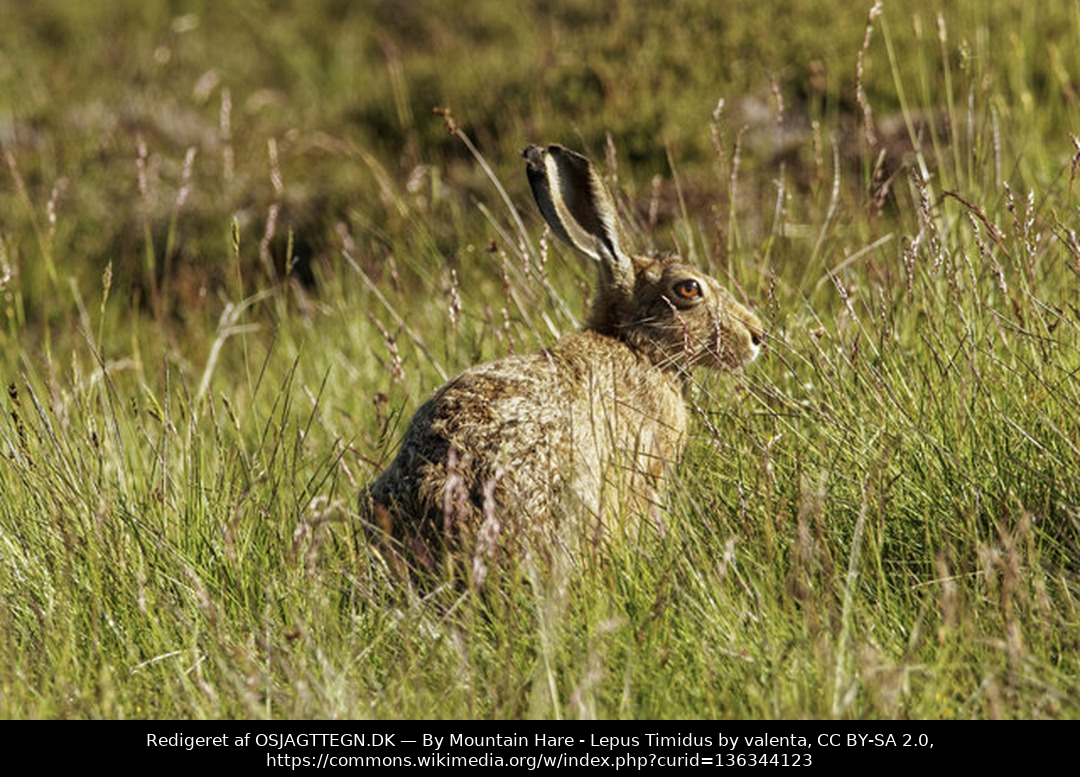
\includegraphics[width=\linewidth, height=7.2cm, keepaspectratio]{Billeder/Dyr/Pattedyr/støttetandede/hare/hare-04.jpg}
  \end{columns}
\end{frame}